\section{Analyse du projet}
Il est probable que vous n'ayez pas besoin d'une autre section dans votre document.
Vous pouvez donc supprimer celle-ci faire remonter toutes les sous-sections et sous-sous-sections d'un cran.
    
    \subsection{Cahier des charges}
        \subsubsection{Description du projet}
            Le groupe a décidé de faire un projet de snake en I4.2 par ce qu'on a pas le choix de faire autre chose.
            Le snake est un jeu qui… blablabla à vous de faire votre description.
        \subsubsection{Liste des fonctionnalités}\label{sssect:fonctionnalites}
            Le rendu final de notre projet comportera les fonctionnalités suivantes:
            \begin{itemize}
                \item Affichage console
                \item Choix de la taille du plateau
                \item Choix de la difficulté
                \item …
            \end{itemize}
            
            Nous avons prévu des fonctionnalités optionnelles, qui ne seront implémentées que s'il nous reste du temps à la fin du semestre:
            \begin{itemize}
                \item Coloration de l'affichage
                \item Jeu multijoueur
                \item Sauvegarde des scores
                \item …
            \end{itemize}
            
            Versions prévues:
            
            V1 (15/04/2020):
            \begin{itemize}
                \item Affichage du plateau
            \end{itemize}
            
            V2:
            \begin{itemize}
                \item …
            \end{itemize}



    \subsection{Conception globale}
        Cette section présente la conception globale du programme implémentant les fonctionnalités données en section~\ref{sssect:fonctionnalites}.
        L'analyse descendante correspondante est donnée en figure~\ref{fig:AD}.
        
        \begin{figure}[!ht]
            \centering % Centre horizontalement tout ce qui est dans l'environnement ``figure''
                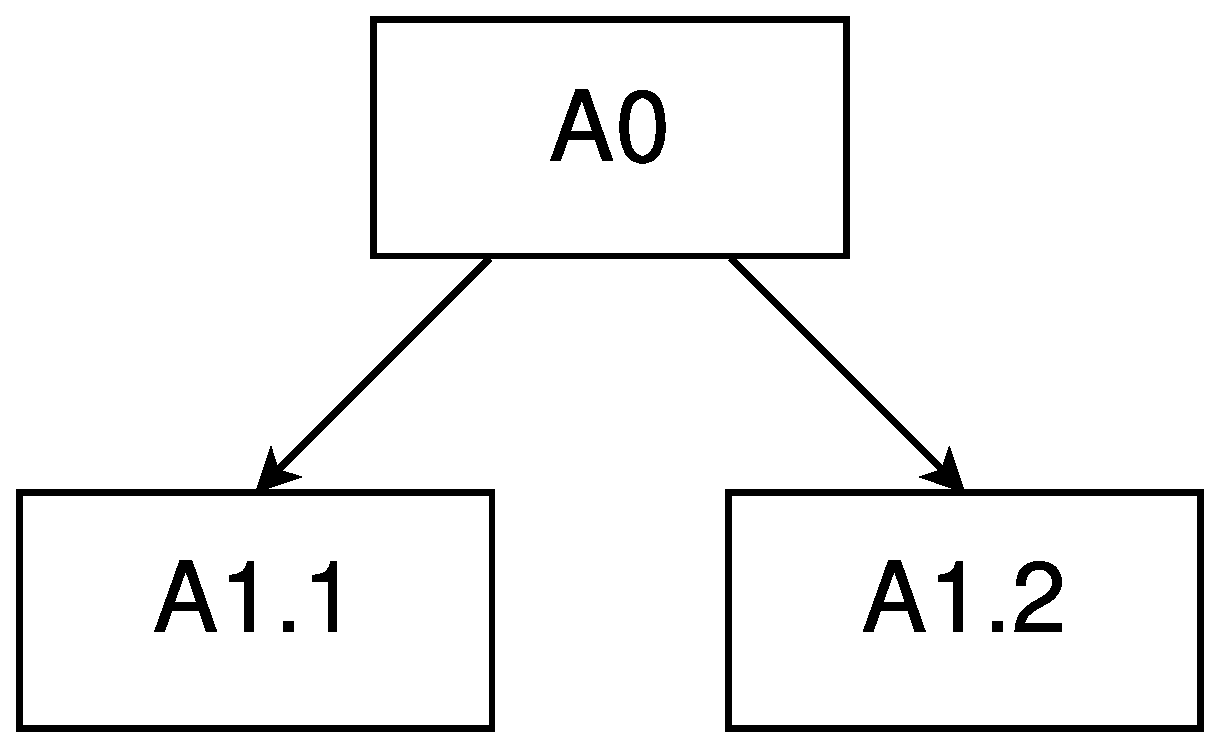
\includegraphics[width=0.5\textwidth]{images/AD.eps} % Chemin vers l'image à ajouter
            \caption{Analyse descendante du projet.} % Légende de l'image
            \label{fig:AD} % Étiquette pour y faire référence ailleurs dans le document
        \end{figure}
        
        Je vous invite à utiliser le programme dia\footnote{\url{https://fr.wikipedia.org/wiki/Dia_(logiciel)}} pour réaliser votre analyse descendante et vos autres diagrammes.
        Le format \verb|.eps| est un très bon choix pour exporter les diagrammes faits avec ce programme étant donné qu'il est vectoriel et très bien géré par \LaTeX{}.
    
    \subsection{Conception préliminaire}
        Le contenu de cette section présente la signature des fonctions et procédures de l'analyse descendante, en précisant les entrées, sorties et entrées/sorties.
        Il peut être intéressant de détailler la signature de certaines fonctions pour justifier certains de vos choix.
        
        Les types personnalisés employés doivent aussi être présentés et défendus dans cette section.
        
    \subsection{Conception détaillée}
        Pour vous aider à écrire des algorithmes propres en \LaTeX{} un paquet spécifique (\verb|algorithm2e|) a été ajouté par défaut à ce modèle de rapport.
        Il vous permet d'inclure du pseudo-code dans votre document pour détailler les algorithmes importants de votre programme.
        Voici un exemple d'un algorithme tiré du projet de morpion du cours d'I2:
        
        \begin{algorithm}[H]
            \SetAlgoLined
            \Fun{aGagne(g :  Grille): Emplacement}{
            \Sortie{s'il n'y a aucun gagnant, l'emplacement renvoyé est l'emplacement vide (\_), sinon c'est l'emplacement représentant la couleur du gagnant (X ou O).}
            \Donnees{i, j: Entier, vainqueur: Emplacement}
            
            vainqueur $\leftarrow$ \_\;
            
            \tcp{lignes}
            \Pour{i $\leftarrow$ 1 à 3}{
                \Si{(g[i][1] = g[i][2]) et (g[i][1] = g[i][3])}{
                    vainqueur $\leftarrow$ g[i][1]\;
                }
            }
            \tcp{colonnes}
            \Pour{j $\leftarrow$ 1 à 3}{
                \Si{(g[1][j] = g[2][j]) et (g[1][j] = g[3][j])}{
                    vainqueur $\leftarrow$ g[1][j]\;
                }
            }
            
            \tcp{diagonales}
            \Si{((g[2][2]= g[1][1]) et (g[2][2]= g[3][3])) ou\\ 
                ((g[2][2]= g[1][3]) et (g[2][2]= g[3][1]))}{
                vainqueur $\leftarrow$ g[2][2]\;
            }
            
            \Retour{vainqueur}
            
            }
            \caption{recherche d'un gagnant dans une grille de Morpion}
        \end{algorithm}
        
        Le mot-clé \enquote{\textbf{Données}} est utilisé pour déclarer les variables utilisées dans l'algorithme.
        
        La documentation du paquet \LaTeX{} pour écrire des algorithmes (\verb|algorithm2e|) est disponible à l'adresse suivante: \url{http://ctan.mines-albi.fr/macros/latex/contrib/algorithm2e/doc/algorithm2e.pdf}(voir notamment la p.41 et les suivantes pour les mots-clés a utiliser pour écrire votre algo en français).
        J'ai implémenté en plus du paquet de base les commandes \verb|\fun{}{}| pour les fonctions et \verb|\proc{}{}| pour les procédures.
        Ces commandes prennent en premier paramètre le nom de la fonction et ses paramètres et en second paramètre le corps de la fonction.
    \subsection{Implémentation}
        Il est aussi possible en \LaTeX{} d'inclure du code source dans un document.
        
        \begin{lstlisting}[language=Pascal,frame=single,caption=code source de la fonction aGagne.]
function aGagne(g :  Grille):Emplacement;
var i,j : Integer; vainqueur: Emplacement;
begin
   vainqueur := _;

   {lignes}
   for i := 1 to 3 do
   	 if (g[i][1] = g[i][2]) and (g[i][1] = g[i][3]) then 
		vainqueur := g[i][1];
	
   {colonnes}
   for j := 1 to 3 do
   	 if (g[1][j] = g[2][j]) and (g[1][j] = g[3][j]) then 
		vainqueur := g[1][j];
   
   {diagonales}   
   if ((g[2][2]= g[1][1]) and (g[2][2]= g[3][3])) or
		((g[2][2]= g[1][3]) and (g[2][2]= g[3][1])) then
			vainqueur := g[2][2];
   aGagne := vainqueur;
end;
        \end{lstlisting}
